\documentclass{beamer} 
\usepackage{amsmath} 
\usepackage{xcolor} 
\usepackage{xpatch} 
\usepackage{cancel} 
\usepackage{enumitem} 
\usepackage{pgfplots}
\usepackage{framed}
\title{End Behavior of Polynomials} 
\pgfplotsset{width = 10cm, compat = 1.9}
\usepgfplotslibrary{external, groupplots}
\tikzexternalize


\begin{document}
	\frame{
	\titlepage
}
	\frame{
		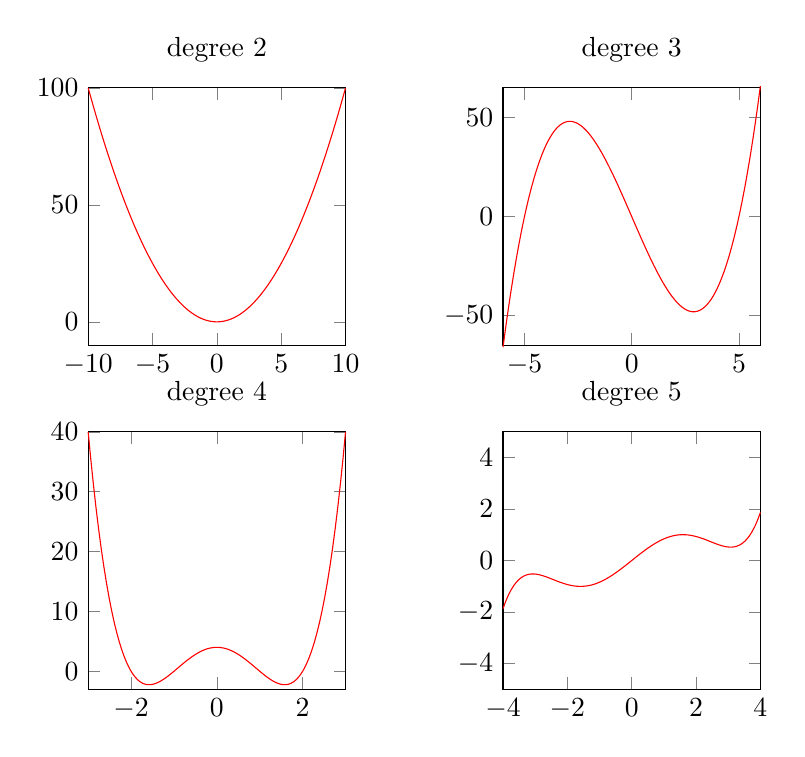
\begin{tikzpicture}
   \begin{groupplot}[
        group style = {group size = 2 by 2, vertical sep = 1.1cm, horizontal sep = 2cm},
        width=0.4\linewidth,
        height=0.4\linewidth,
        ]

        \nextgroupplot[
                title = degree 2,
                xmin = -10,
                xmax = 10,
                ymin = -10,
                ymax = 100,
                ymode = linear,
                clip = false,
        ]
        \addplot [
		domain = -10:10,
		samples = 100,
		color = red,
		]
	   {x^2};

        \nextgroupplot[
                title = degree 3,
                xmin = -6,
                xmax = 6,
                ymin = -65,
                ymax = 65,
                ymode = linear,
                clip = false,
        ]
        \addplot [
		domain = -6:6,
		samples = 100,
		color = red,
		]
	   {x*(x - 5)*(x + 5)};

        \nextgroupplot[
                title = degree 4,
                xmin = -3,
                xmax = 3,
                ymin = -3,
                ymax = 40,
                ymode = linear,
                clip = false,
        ]
        \addplot [
		domain = -3:3,
		samples = 100,
		color = red,
		]
	   {(x - 2)*(x - 1)*(x + 1)*(x + 2)};
        \nextgroupplot[
                title = degree 5,
                xmin = -4,
                xmax = 4,
                ymin = -5,
                ymax = 5,
                ymode = linear,
                clip = false,
        ]
        \addplot [
		domain = -4:4,
		samples = 100,
		color = red,
		]
	   {x-(x^3/6) + x^5 / 120};
   \end{groupplot}
\end{tikzpicture}

	
}
	\frame{
		\begin{tikzpicture}
\begin{axis}[
    axis lines = left,
    xlabel = $x$,
    ylabel = {$f(x)$},
]

%Single point
\addplot[domain = -10:10, mark = *, color = green] coordinates {(0,0)};
\addplot[domain = -10:10, mark = *, color = green] coordinates {(1,1)};
\addplot[domain = -10:10, mark = *, color = green] coordinates {(2,4)};
\addplot[domain = -10:10, mark = *, color = green] coordinates {(3,9)};
\addplot[domain = -10:10, mark = *, color = green] coordinates {(4,16)};
\addplot[domain = -10:10, mark = *, color = green] coordinates {(5,25)};
\addplot[domain = -10:10, mark = *, color = green] coordinates {(6,36)};
%red parabola
\addplot [
    domain=-10:10,
    samples=100,
    color=red,
]
{x^2};
\addlegendentry{$x^2$}
\end{axis}
\end{tikzpicture}

\\\pause
		$x\rightarrow \infty$ \pause \hspace{1cm} $f(x) \rightarrow \infty$
		$\hspace{1cm}x\rightarrow -\infty$ \pause \hspace{1cm} $f(x) \rightarrow \infty$
}
	\frame{
		\begin{tikzpicture}
\begin{axis}[
    axis lines = left,
    xlabel = $x$,
    ylabel = {$f(x)$},
]
%red parabola
\addplot [
    domain=-6:6,
    samples=100,
    color=red,
]
{x*(x - 5)*(x + 5)};
\addlegendentry{$x^3 - 25x$}
\end{axis}
\end{tikzpicture} 
\\\pause
		$x\rightarrow \infty$ \pause \hspace{1cm} $f(x) \rightarrow \infty$
		$\hspace{1cm}x\rightarrow -\infty$ \pause \hspace{1cm} $f(x) \rightarrow -\infty$
}
\end{document}
